% !Mode:: "TeX:UTF-8"

\chapter{数据来源与数据预处理}
\label{chap:theory}

\section{数据来源}

本文采用了两个不同的数据集进行实验,通过使用这两个数据集,验证模型在不同数据集上的泛化能力和有效性。在实验过程中,对这两个数据集进行数据预处理。通过对这些数据的充分利用,能够提高模型的性能和准确度,进一步探究这些数据集的内在特性和规律。

数据集1中协同得分数据源自O'Neil团队发布的高通量协同筛查数据\cite{17}(下称数据集1为O'Neil数据集),涵盖了来自七种不同组织的39个癌细胞系和38种药物(24种批准药物和 14种试验药物)。其中,22种药物(14种试验药物和8种批准药物,统称为穷举组药物)两两组合(不考虑药物自身的组合,不考虑药物组合的顺序,以下同),得到231种药物组合,剩余的16种批准药物(统称为补充组药物)与22种穷举组药物组合,构成352种药物组合,总计583种药物组合。部分数据展示如表~\ref{tb:ms}所示。

% \begin{table}[htbp]
%   \centering
%   \caption{文件583drugs39cellsynergy.xlsx的部分数据展示}
%   \label{tb:ms}
%   \begin{tabular}{llrrrrrrrrr}
%     \toprule
%     DrugA & DrugB & A2058 & A2780 & A375 & A427 & CAOV3 &  ... \\
%     \midrule
%     MK-5108 & SORAFENIB & -9.50 & 2.60 & 15.16 & 6.22 & -16.35 & ... \\
%     VINORELBINE & SUNITINIB & -13.16 & -4.03 & 11.05 & 10.46 & -15.57 & ... \\
%     SUNITINIB & MK-8776 & 26.42 & 14.48 & 29.51 & 17.51 & 17.73 & ... \\
%     % 5-FU & DINACICLIB & 4.33 & -8.16 & -5.41 & -7.74 & -14.34 & ... \\
%     % SUNITINIB & MK-2206 & 42.28 & 22.49 & 12.96 & 15.56 & 10.48 & ... \\
%     \multicolumn{8}{l}{...} \\
%     \bottomrule
%   \end{tabular}
% \end{table}

\begin{table}[htbp]
  \centering
  \caption{O'Neil数据集协同得分的部分数据展示}
  \label{tb:ms}
  \small
  \begin{tabular}{p{2.5cm} p{2.4cm} p{1.2cm} p{1.2cm} p{1.1cm} p{1cm} p{1.2cm} p{0.5cm}}
    \toprule
    DrugA & DrugB & A2058 & A2780 & A375 & A427 & CAOV3 &  ... \\
    \midrule
    MK-5108 & SORAFENIB & -9.50 & 2.60 & 15.16 & 6.22 & -16.35 & ... \\
    VINORELBINE & SUNITINIB & -13.16 & -4.03 & 11.05 & 10.46 & -15.57 & ... \\
    SUNITINIB & MK-8776 & 26.42 & 14.48 & 29.51 & 17.51 & 17.73 & ... \\
    5-FU & DINACICLIB & 4.33 & -8.16 & -5.41 & -7.74 & -14.34 & ... \\
    % SUNITINIB & MK-2206 & 42.28 & 22.49 & 12.96 & 15.56 & 10.48 & ... \\
    % \multicolumn{8}{l}{...} \\
    ... & ... & ... & ... & ... & ... & ... & ... \\
    \bottomrule
  \end{tabular}
\end{table}

\begin{table}[htbp]
\centering
\caption{O'Neil数据集药物分子指纹的部分数据展示\label{tb:md}}
\small
\begin{tabular}{p{2.5cm} p{1.2cm} p{1.2cm} p{1.2cm} p{1.2cm} p{1.2cm} p{1.2cm} p{1.2cm}}
\toprule
Drug & FPT1 & FPT2 & FPT3 & FPT4 & FPT5 & FPT6 & ... \\
\midrule
5-FU & 0 & 0 & 0 & 0 & 0 & 0 & ... \\
ABT-888 & 0 & 0 & 0 & 0 & 0 & 0 & ... \\
AZD1775 & 0 & 0 & 0 & 0 & 0 & 0 & ... \\
BEZ-235 & 0 & 0 & 0 & 0 & 0 & 0 & ... \\
% BORTEZOMIB & 0 & 0 & 0 & 0 & 0 & 0 & ... \\
% CARBOPLATIN & 0 & 0 & 1 & 0 & 1 & 0 & ... \\
... & ... & ... & ... & ... & ... & ... & ... \\
\bottomrule
\end{tabular}
\end{table}

为了表征单个药物的化学结构,本文使用了166个结构特征的MACCS指纹,该指纹数据源自参考文献\cite{16}的补充材料,表~\ref{tb:md}中展示了部分数据,指纹数据由0和1表示该结构特征。先前的研究\cite{16}发现,与药物靶标谱相比,药物分子指纹对于药物组合敏感性评分(CSS)的预测能力较差,这表明使用MACCS指纹捕获相关结构信息以预测药物组合敏感性可能不是最佳选择。然而,考虑到本文的重点是验证相似性网络模型在协同得分预测方面的有效性,这些药物分子指纹数据对实验研究依然具有意义。

数据集2来源于文献\cite{18}的补充材料,原始数据来自美国国家癌症研究所生成的NCI-ALMANAC数据集(下称数据集2为NCI-ALMANAC数据集),这是迄今为止最大的可用药物组合数据集,涵盖了大约100种小分子药物的5000多个组合,针对60种细胞进行了筛选,含有超过300万个反应测量值的各浓度线。该数据集包括的药物是FDA批准的肿瘤药物,具有经证实的活性和既定的安全特征。本文在文献\cite{18}的基础上,经过剔除重复测量值后,选取最后一次测量的数据结果,并将其提取和整合为以下两部分:50种药物分子指纹(指纹数据由0和1表示该结构特征)、587个药物组合与60个细胞系的协同得分。部分数据展示如表~\ref{tb:ndd},表~\ref{tb:ns}所示。

% \begin{figure}[htbp!]
% \centering
% 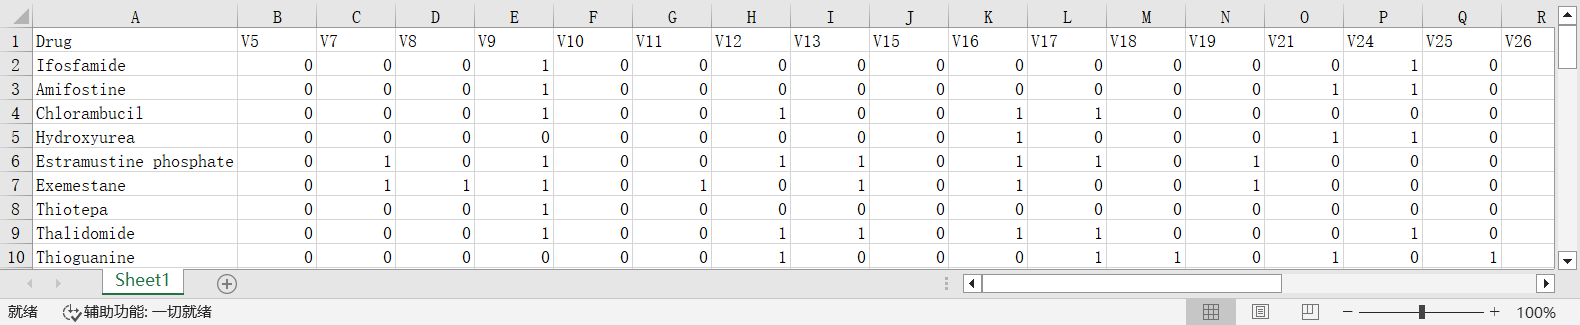
\includegraphics[width=0.8\textwidth]{3}
% \caption{文件50种药物分子指纹.xlsx的部分数据展示\label{fig:ndd}}
% \end{figure}

\begin{table}[htbp]
\centering
\caption{NCI-ALMANAC数据集药物分子指纹的部分数据展示\label{tb:ndd}}
\small
\begin{tabular}{p{2.5cm} p{1.2cm} p{1.2cm} p{1.2cm} p{1.2cm} p{1.2cm} p{1.2cm} p{1.2cm}}
\toprule
Drug & V5 & V7 & V8 & V9 & V10 & V11 & ... \\
\midrule
Ifosfamide & 0 & 0 & 0 & 1 & 0 & 0 & ... \\
Amifostine & 0 & 0 & 0 & 1 & 0 & 0 & ... \\
Chlorambucil & 0 & 0 & 0 & 1 & 0 & 0 & ... \\
Hydroxyurea & 0 & 0 & 0 & 0 & 0 & 0 & ... \\
% Estramustine phosphate sodium & 0 & 1 & 0 & 1 & 0 & 0 & ... \\
% Exemestane & 0 & 1 & 1 & 1 & 0 & 1 & ... \\
% Thiotepa & 0 & 0 & 0 & 1 & 0 & 0 & ... \\
... & ... & ... & ... & ... & ... & ... & ... \\
\bottomrule
\end{tabular}
\end{table}

\begin{table}[htbp]
\centering
\caption{NCI-ALMANAC数据集协同得分的部分数据展示\label{tb:ns}}
\small
\begin{tabular}{p{2.5cm} p{2.5cm} p{1.4cm} p{1.4cm} p{1.4cm} p{1.4cm} p{0.5cm}}
\toprule
DrugA & DrugB & 786-0 & A498 & A549 & ACHN & ... \\
\midrule
Ifosfamide & Chlorambucil & -277.60 & -266.71 & -245.81 & -240.25 & ... \\
Amifostine & Ifosfamide & -323.37 & -310.81 & -286.64 & -281.03 & ... \\
Amifostine & Chlorambucil & -176.69 & -259.98 & -267.98 & -209.61 & ... \\
Chlorambucil & Exemestane & -98.88 & -182.90 & -179.01 & -177.18 & ... \\
% Hydroxyurea & Chlorambucil & -217.29 & -269.98 & -228.54 & -136.28 & ... \\
... & ... & ... & ... & ... & ... & ... \\
\bottomrule
\end{tabular}
\end{table}

% \begin{figure}[htbp!]
% \centering
% 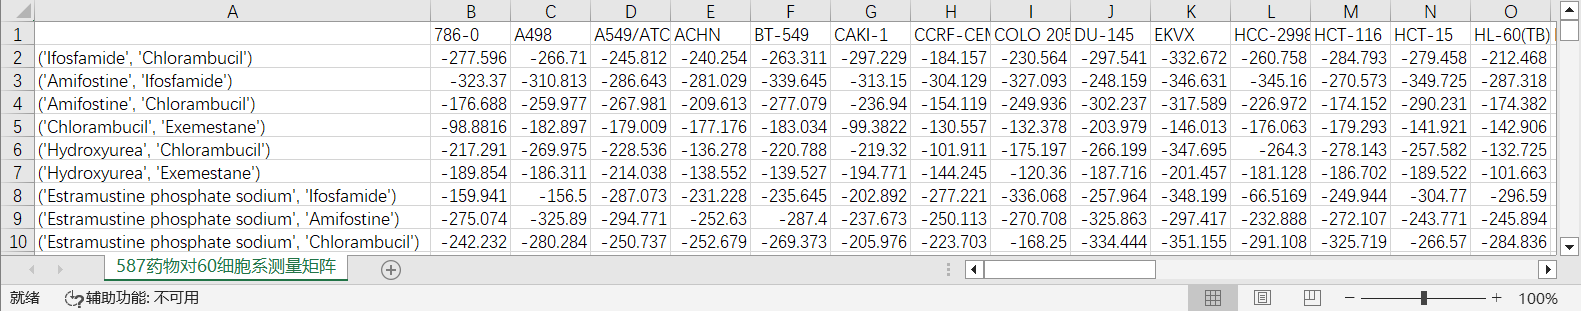
\includegraphics[width=0.8\textwidth]{4}
% \caption{文件587药物组合60细胞系测量矩阵.csv的部分数据展示\label{fig:ns}}
% \end{figure}

\section{数据预处理}

在类似于本文的相关研究中,通常使用原始数据进行模型的构建和求解。例如,岭回归方法要求目标矩阵的核范数最小并且接近原始矩阵,因此无需对原始数据进行标准化处理。而随机森林则是一种基于决策树的集成学习方法,它可以通过随机选择子样本和特征来构建多个决策树,并使用这些决策树的预测结果进行集成。由于随机森林是基于树的模型,不会受到数据缩放的影响,因此也无需对原始数据进行标准化处理。

\begin{figure}
\centering
  \begin{minipage}{0.45\linewidth}
    \centering
    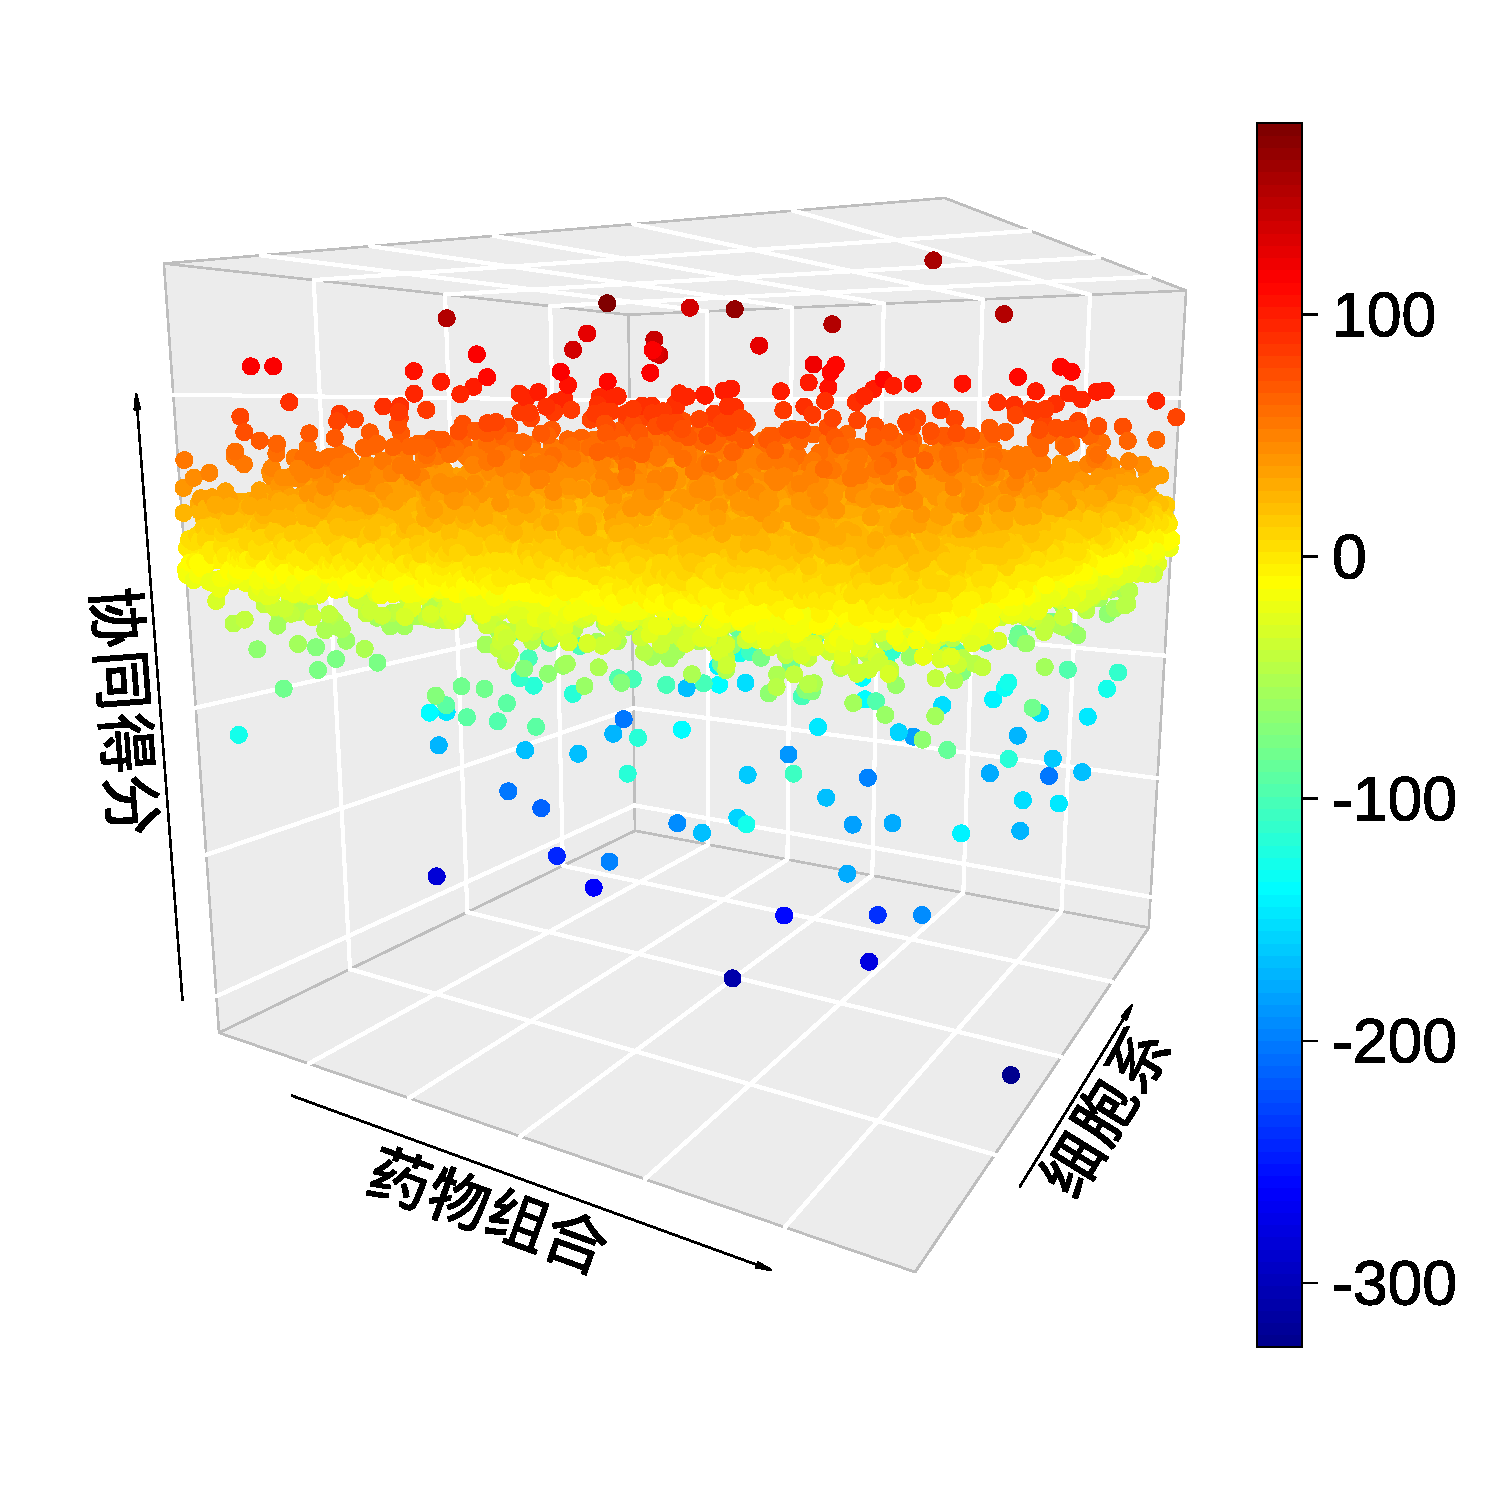
\includegraphics[width=\linewidth]{figures/old_o.pdf}
    \caption{基于O'Neil数据集\\协同得分的原始数据分布}
    \label{fig:sub1}
  \end{minipage}%
  \begin{minipage}{0.45\linewidth}
    \centering
    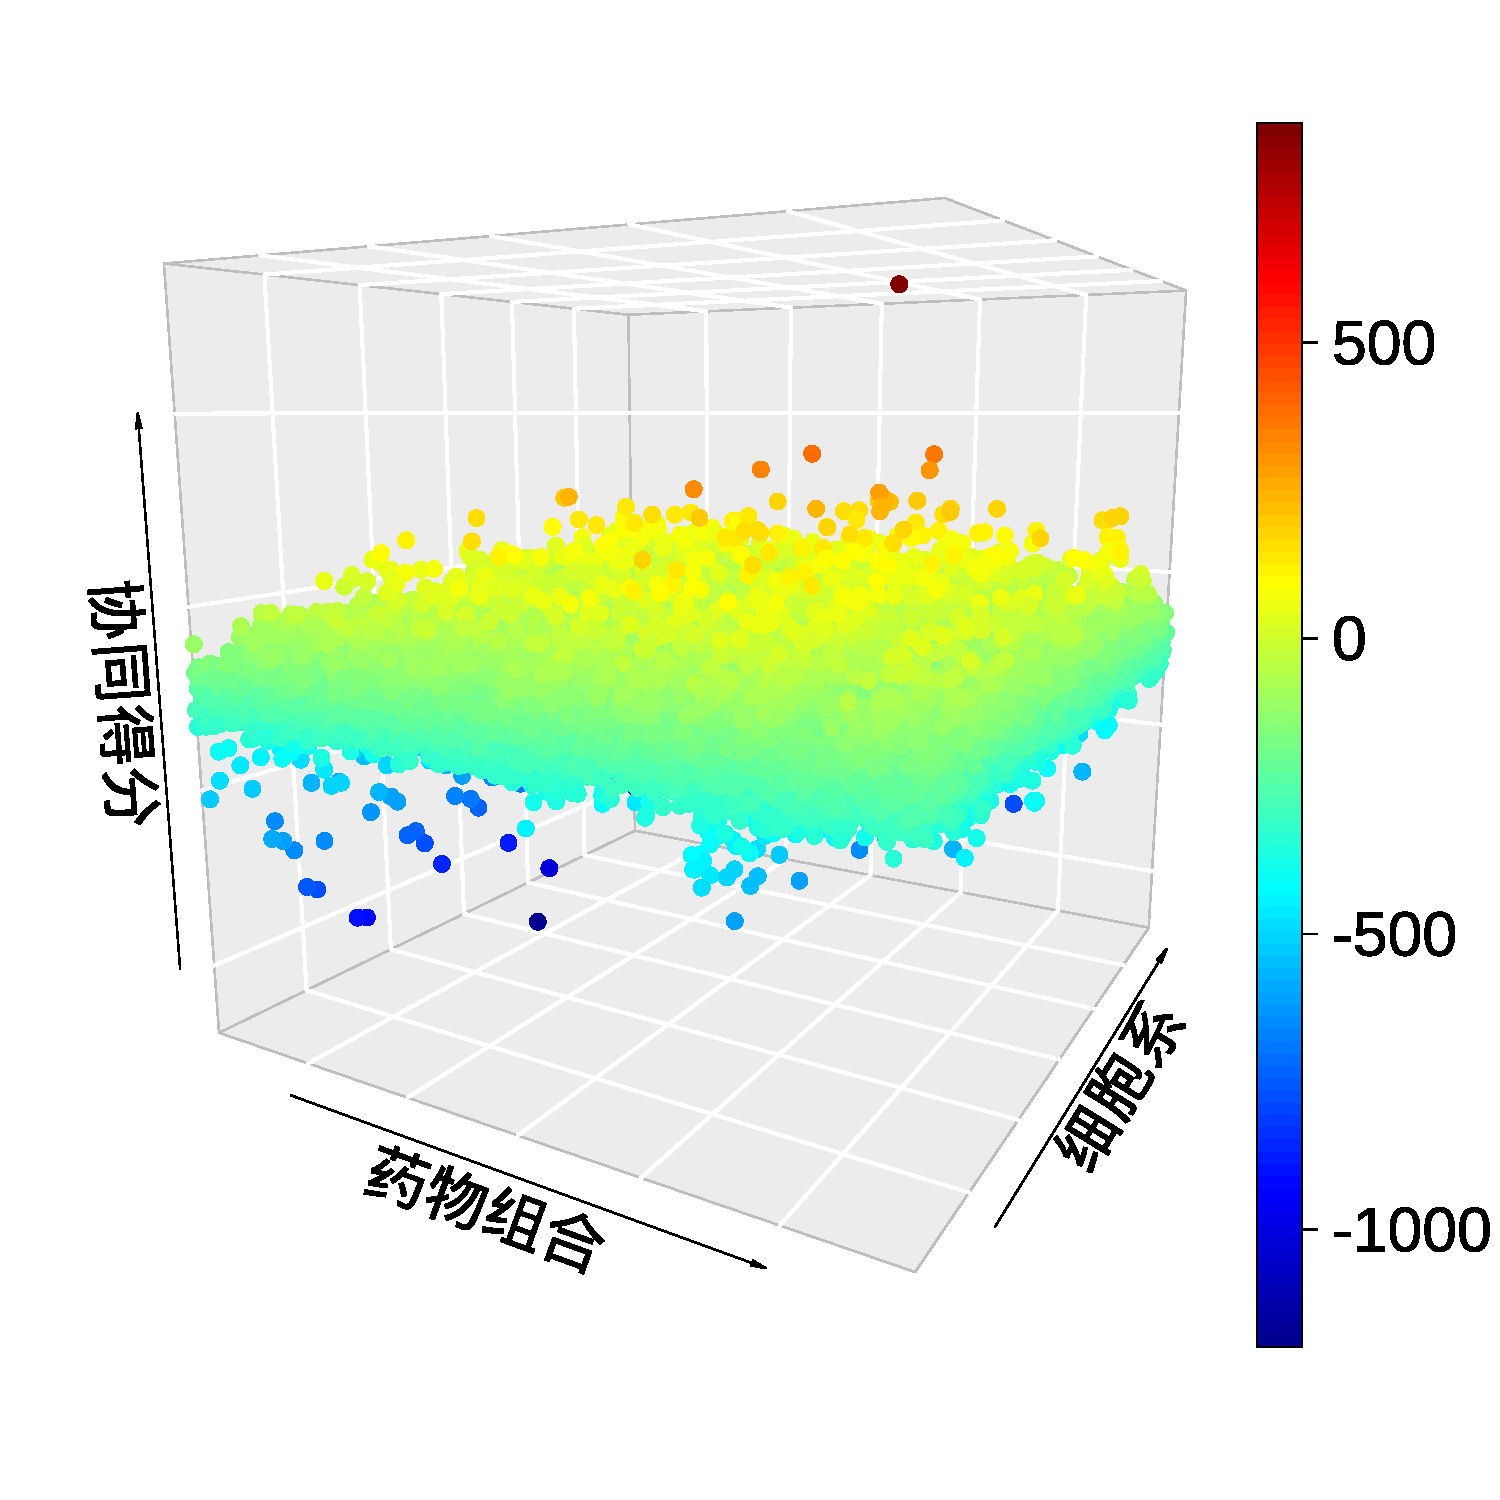
\includegraphics[width=\linewidth]{figures/new_o.pdf}
    \caption{基于NCI-ALMANAC数据集\\协同得分的原始数据分布}
    \label{fig:sub3}
  \end{minipage}
\end{figure}

本文需要使用基于高斯核函数扩展的权重函数来预测各目标药物组合的协同得分,需要使用高相似的药物组合的协同得分来预测目标药物组合的协同得分。图~\ref{fig:sub1}和图~\ref{fig:sub3}展示了本文的原始数据集中的协同得分部分,经过观察,可以发现在原始数据集中,大部分数据都分布在中间范围内,但同时也存在一些数据的测量结果明显偏大或偏小,分布不均匀有极端值。当原始数据的差异较大时,部分高相似的药物组合的权重会过高,从而影响预测结果。因此,在使用前需要对原始数据进行标准化处理\supercite{20}。

本文对两个数据集中的协同得分进行了Z-score行标准化处理,让标准化后的数据具有相同的均值和标准差,以使得不同药物组合之间的值具有可比性,方便数据的比较和分析。如果不进行Z-score行标准化处理,部分数据的数值差异过大,也会影响到后续的相似性系数计算结果。在计算Tanimoto相关系数时,奇异值可能会影响排名的计算,从而影响系数的计算结果。在计算Spearman相关系数时,数据集中存在极端值或异常值可能会导致计算得到的排名与实际情况不符,从而影响计算结果。

\begin{equation}
z_{ij} = \frac{x_{ij} - \mu_j}{\sigma_j}.
\end{equation}

\noindent 其中,$x_{ij}$ 是第 $i$ 行第 $j$ 列的数据,$\mu_j$ 是第 $j$ 列的均值,$\sigma_j$ 是第 $j$ 列的标准差,$z_{ij}$ 是标准化后的第 $i$ 行第 $j$ 列的值。对于每一列数据,先计算出其均值 $\mu_j$ 和标准差 $\sigma_j$,然后用上述公式将每一行的数据进行标准化。标准化后的数据满足均值为0,标准差为1的正态分布。

\newpage

\begin{figure}
\centering
  \begin{minipage}{0.45\linewidth}
    \centering
    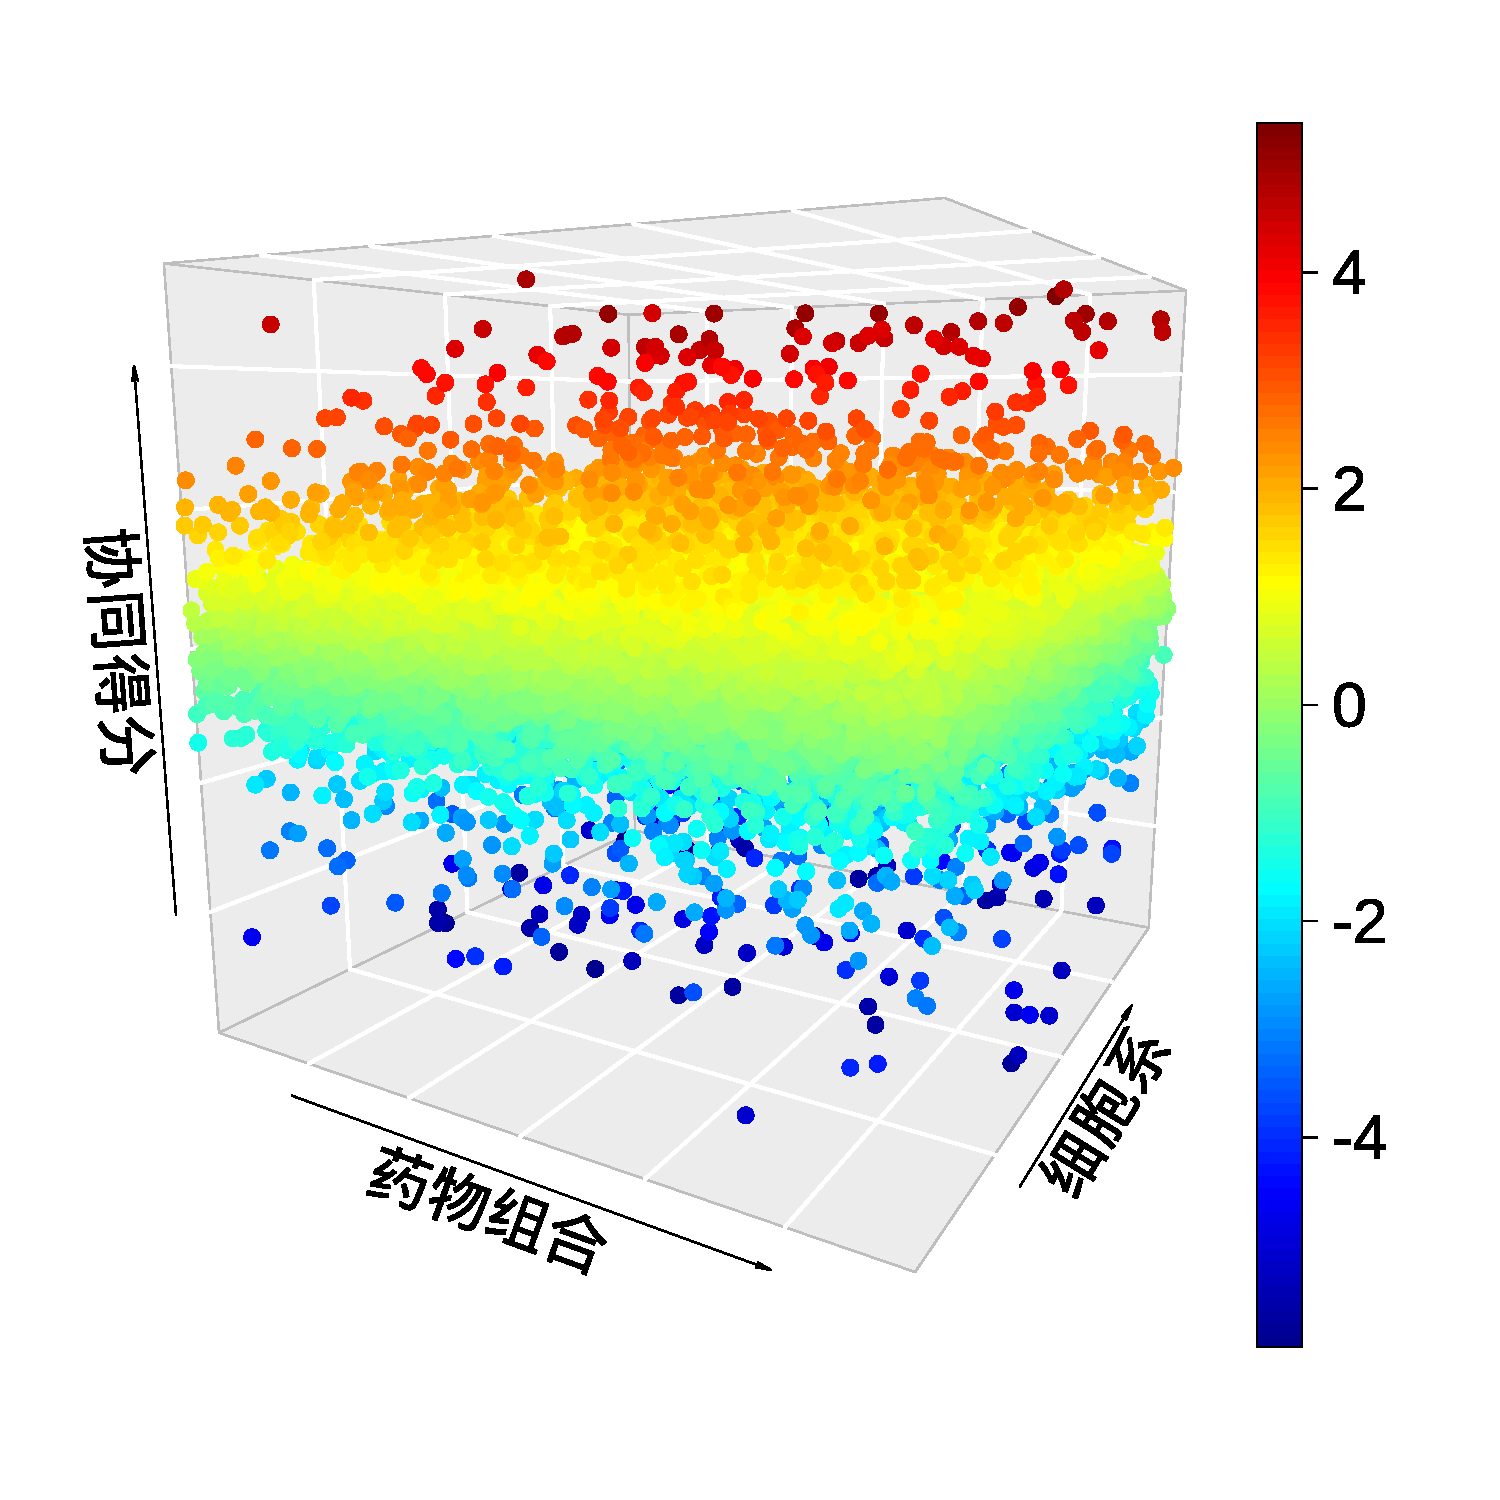
\includegraphics[width=\linewidth]{figures/old_n.pdf}
    \caption{基于O'Neil数据集\\协同得分标准化后的数据分布}
    \label{fig:sub2}
  \end{minipage}%
  \begin{minipage}{0.45\linewidth}
    \centering
    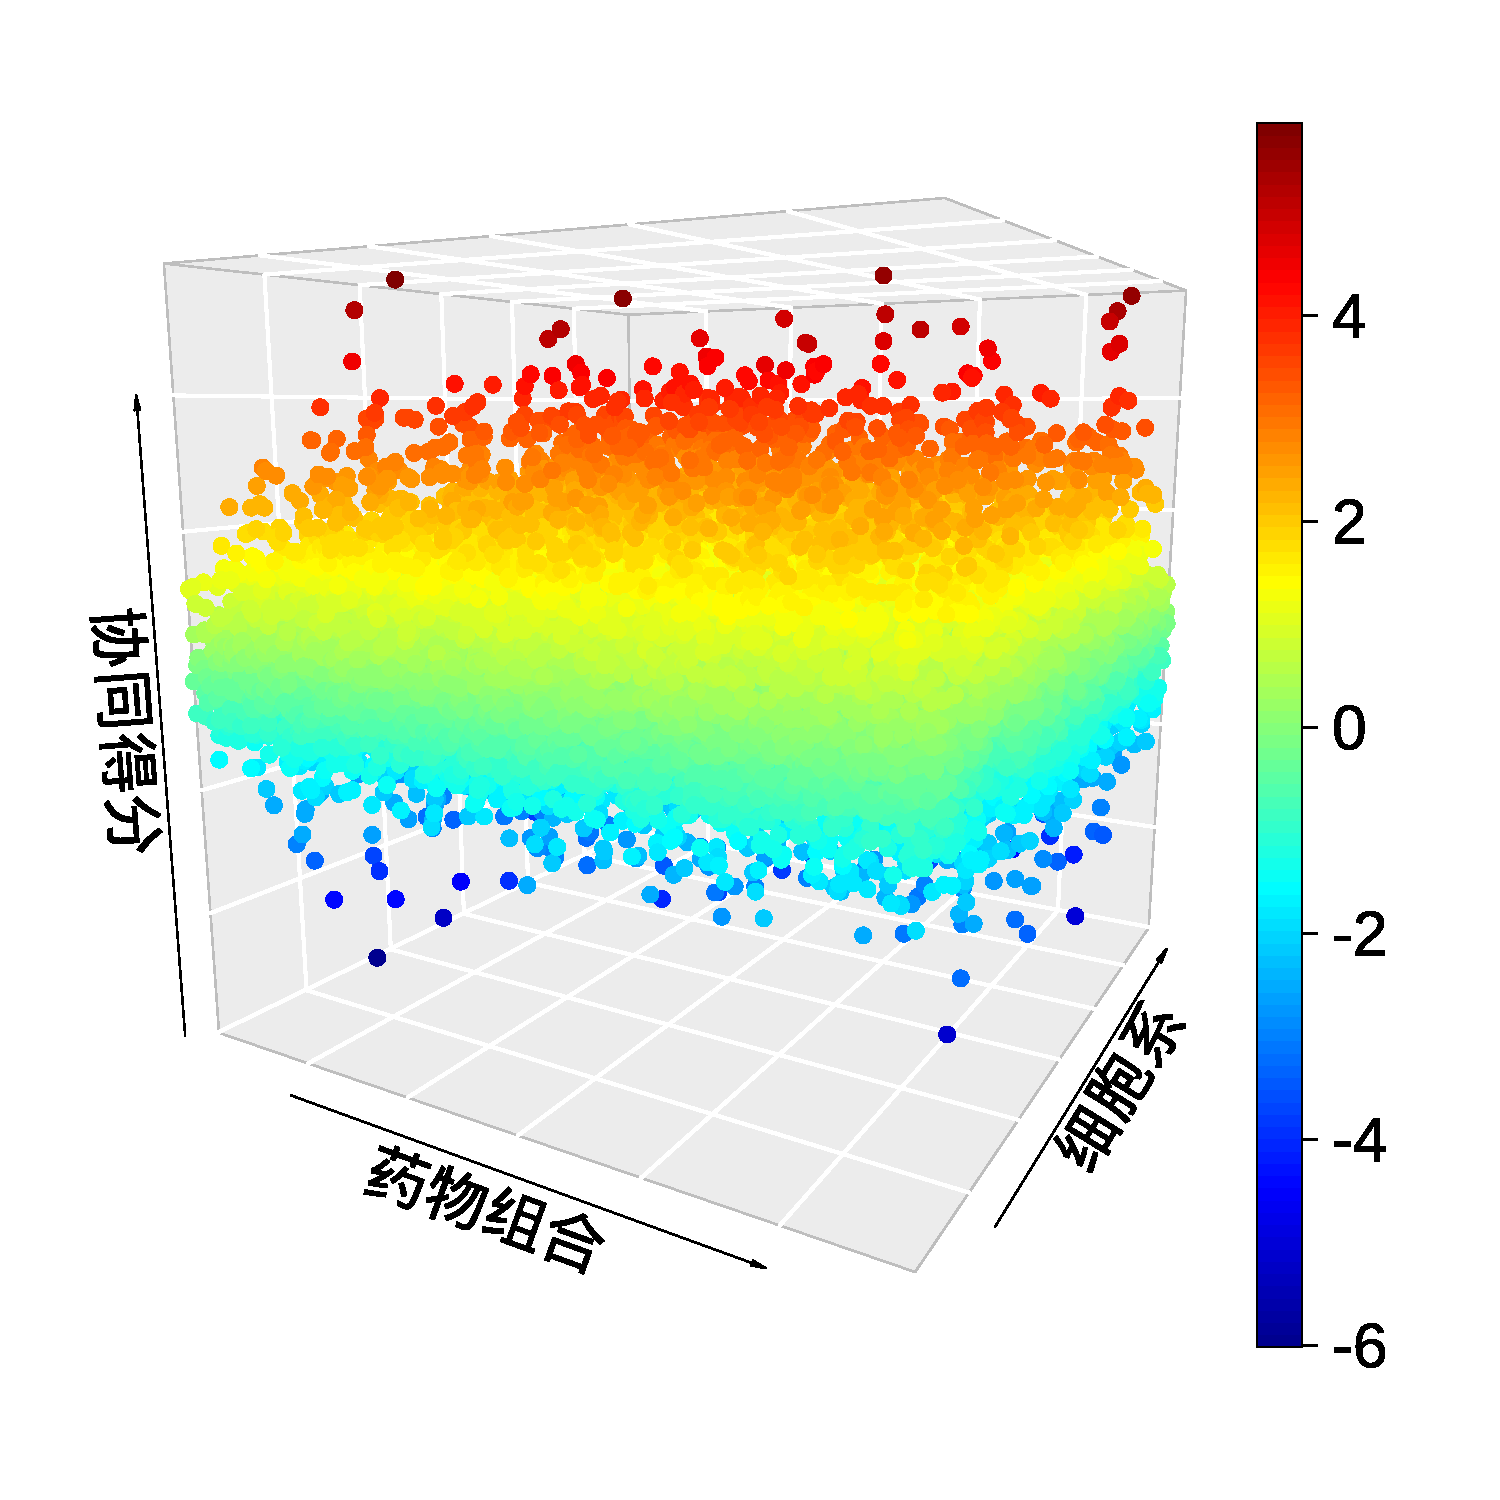
\includegraphics[width=\linewidth]{figures/new_n.pdf}
    \caption{基于NCI-ALMANAC数据集\\协同得分标准化后的数据分布}
    \label{fig:sub4}
  \end{minipage}
\end{figure}

图~\ref{fig:sub2}和图~\ref{fig:sub4}展示了本文的标准化后数据集中的协同得分部分。对于经过预处理的数据集,由于经过了标准化处理,数据分布变得更加均匀了,这表明数据已经成功地去除了初始的偏差。使用预处理后的数据进行后续的模型构建和求解,将不再出现因某一药物权重过高而导致模型偏差的现象,模型的预测效果更为准确。

\section{本章小结}

本章主要介绍了前期工作中所采用的数据集和数据预处理方法。研究使用了O'Neil数据集和NCI-ALMANAC数据集进行实验,以验证提出的模型在不同数据集上的泛化能力和有效性。数据集的处理包括对O'Neil数据集和NCI-ALMANAC数据集中的协同得分进行Z-score行标准化处理,以确保数据具有可比性和一致性。这些处理能够提高模型的性能和准确度,并深入研究这些数据集的特性和规律。